\documentclass[10pt,twocolumn]{article}
\usepackage[letterpaper,margin=0.75in,columnsep=0.24in]{geometry}
\usepackage{mathptmx,amsmath,amssymb,graphicx,booktabs,microtype,url}
\usepackage[font=small,labelfont=bf]{caption}
\usepackage[hidelinks]{hyperref}
\usepackage{fancyhdr}
\pagestyle{fancy}\fancyhf{}
\fancyhead[L]{\small SCARA simulation study}
\fancyhead[R]{\small Passive learning and probe costs}
\fancyfoot[C]{\thepage}
\setlength{\headheight}{14pt}
\setlength{\parskip}{2pt}
\raggedbottom
\title{\vspace{-1.3em}\LARGE\bfseries Payload Probing with Passive Learning:\newline Break-Even and Decision Regret in a SCARA Simulation}
\author{Anonymous authors}
\date{}
\begin{document}
\maketitle\thispagestyle{fancy}
\begin{abstract}
When a robot learns payload parameters during normal work, an extra identification motion is useful only if its downstream savings exceed its execution cost. We study this trade-off in a synthetic four-degree-of-freedom SCARA benchmark with a common integral tracking controller, noisy sensing, online estimation and explicit overhead and failure accounting. The original 1,080 held-out batches are supplemented by 6,050 exploratory post-review batches. With nominal sensing and the specified duration heuristic, probing increases mean robot time through 100-item batches; the conditional excess is 0.796 s for yaw-exciting tasks and 0.311 s for low-yaw tasks at 100 items. Under tenfold sensor noise, a low-yaw 60-item batch instead saves 1.052 s [0.923, 1.194], conditional on nine paired completions. A fixed-mean covariance rollout selects those beneficial probes, but misses beneficial individual nominal scenarios and misclassifies cases near break-even. Doubling the duration margin provides another counterexample to its decision quality. Probe-induced failures under faster excitation and lost uncertainty coverage under friction mismatch remain in the results. The contribution is an auditable accounting benchmark and a bounded regime map, not a generally superior probing policy or a safety guarantee.
\end{abstract}
\noindent\textbf{Keywords:} payload identification; SCARA; passive learning; batch scheduling; decision regret; reproducibility.

\section{Introduction}
Payload properties influence feedforward control and the duration at which a manipulator can execute a transfer. A separate excitation motion can improve parameter estimates, but also consumes time. In a production batch, the relevant question is whether the resulting savings over the remaining items exceed that added time. The comparison changes when ordinary production motions also provide information: the no-probe alternative should not be represented by permanently frozen uncertainty.

This study asks a narrow empirical question: \emph{does one additional wrist probe reduce total batch time relative to an otherwise identical controller that learns during normal work?} The scope is a centered, axisymmetric payload described by mass and yaw inertia, shared across all objects in a batch. We study two prescribed task families and one fixed probe. We do not optimize general excitation trajectories or implement an industrial cell.

Our contribution is a computational accounting benchmark: paired probe/no-probe execution, a competent passive estimator, explicit overhead, and retained failures. We assess a fixed-mean covariance rollout and an illustrative horizon-multiplied ablation, without assuming either is a validated decision algorithm. The original short-batch result is supplemented by larger batches, sensitivity analyses, and two-action hindsight regret. This is a methodological simulation contribution, not a new identification principle or an industrial validation.

\section{Related work and scope of the claim}
Payload estimation from manipulator motion is classical~\cite{atkeson1986}. Online estimation within a tracking controller belongs to adaptive manipulation~\cite{slotine1987}; our projected integral-regression estimator is not their adaptive law and inherits none of its theoretical guarantees. Dedicated excitation design also predates this work~\cite{swevers1997}. We use one prescribed probe rather than optimizing an excitation trajectory.

Application-oriented experiment design connects model accuracy to control performance~\cite{hjalmarsson2005}. Bombois et al.~\cite{bombois2006} explicitly minimize identification cost, including experiment duration and performance degradation. They also identify conditions in which sufficiently long normal closed-loop operation can supply the required information without external excitation. Thus the principle that passive information can remove the need for a separate experiment is established; our contribution is a bounded batch-time case study.

Feng and Jiang couple tracking and experiment design~\cite{feng2020}. Vantilborgh et al.~\cite{vantilborgh2026} optimize task-relevant trajectories through adaptive closed-loop dynamics within a single attempt. Their formulation already accounts for learning during execution. Our fixed-mean, two-action repeated-batch forecast is substantially simpler; no superiority over their algorithm is tested.

Event-triggered learning is established~\cite{solowjow2020}. We add a normalized uncertainty-threshold comparator inspired by the general triggering idea, with an explicitly declared engineering threshold; it is not a reproduction of that paper's communication-driven test. Always-probe provides a fixed-schedule comparator. The horizon-multiplied ablation is only an illustrative omission of future passive learning: we make no claim that prior work uses this exact rule. Zhang et al.~\cite{zhang2025} provide bounded-noise payload identification with safety guarantees absent from our Gaussian simulation. Trajectory time scaling under model uncertainty is also established~\cite{moreno2006}; our duration margin is a specified heuristic, not an optimal-control construction.

\section{Synthetic system and observations}
\subsection{Dynamics and task}
Let $q=[q_1,q_2,z,q_4]^\top$, with $z$ positive upward and tool yaw $\phi=q_1+q_2+q_4$. Using standard Lagrangian construction~\cite{lynch2017}, the model is
\begin{equation}
 M(q,\theta)\ddot q+c(q,\dot q,\theta)+g(\theta)+f(\dot q)=\tau,
\end{equation}
where $\theta=[m_p,J_p]^\top$. The payload is centered on the vertical tool axis. Link lengths are 0.35 and 0.25 m, link masses 3 and 2 kg, carriage mass $m_c=0.8$ kg, and unloaded wrist inertia $J_{w0}=0.008$ kg m$^2$. Rotor inertias are $[0.008,0.004,0,0.001]$ in the corresponding joint units. Horizontal links are uniform rods. Smooth friction is $f_i=b_i\dot q_i+d_i\tanh(\dot q_i/0.02)$, with $b=[0.08,0.06,2,0.01]$ and $d=[0.03,0.025,0.1,0.005]$ in SI joint units. The mass contribution is $m_p J_v(q)^\top J_v(q)$, where $J_v$ is the tool translational Jacobian; the yaw contribution is $J_p ss^\top$, $s=[1,1,0,1]^\top$. The supplement gives the full matrix and independent energy derivation.

Effort caps are $[25,18,80,3]$, velocity limits $[4,4,0.8,6]$, and acceleration limits $[25,25,5,40]$, using radians and metres as appropriate. Joint bounds are $[-2.8,-2.8,0.02,-2\pi]$ to $[2.8,2.8,0.30,2\pi]$. These are synthetic engineering choices, not a manufacturer's specifications.

A batch consists of $N$ repetitions of a loaded point-to-point transfer and an unloaded return. Each grasp/release includes a commanded 50 ms dwell and a 50 ms completion hold. Physical position and velocity carry between segments. The payload changes instantaneously at the beginning of grasp/release; gripper contact, approach waypoints and obstacle avoidance are omitted. The nominal start is $[-0.65,1.15,0.10,-0.50]$ and goal $[0.45,0.75,0.18,0.20]$. The first two goal joints vary independently by $\pm0.06$ rad. The low-yaw family modifies $q_4$ to produce a net yaw change of 0.15 rad; the other family retains the nominal wrist goal.

\subsection{Common controller and sensor model}
All methods use the same saturated computed-torque controller:
\begin{align}
 u&=\ddot q_r+\Omega^2e+2\Omega\dot e+k_0\Omega^2\eta,\\
 \tau&=\operatorname{sat}\{M(q_m,\hat\theta)u+c(q_m,\dot q_m,\hat\theta)
 \nonumber\\[-2mm]
 &\hspace{25mm}+g(\hat\theta)+f(\dot q_m)\},
\end{align}
where $\Omega=\operatorname{diag}(18,20,30,24)$ s$^{-1}$, $k_0=6$ s$^{-1}$, and $\eta$ integrates position error. It is clipped to $\pm0.02$ rad s for rotational joints and $\pm0.02$ m s for the vertical joint, frozen when any effort saturates, and reset at each segment transition. Including integral compensation prevents the fixed-parameter comparator from being handicapped solely by a persistent gravity-compensation offset. The reference uses $q_r=q_a+(q_b-q_a)(10r^3-15r^4+6r^5)$, $r=t/T\in[0,1]$, with analytical derivatives and constant endpoints outside this interval. The ideal fixed-model scalar error polynomial is $s^3+2\omega s^2+\omega^2s+k_0\omega^2$; the Routh condition $k_0<2\omega$ holds for all four frequencies. This is not a proof for the saturated adaptive loop. Friction is exactly known only in the nominal runs.

The controller period is 2 ms, with a zero-order-held torque and RK4 plant integration. Independent zero-mean Gaussian position noise has standard deviations $[10^{-5},10^{-5},2\cdot10^{-6},10^{-5}]$; velocity deviations are $[10^{-3},10^{-3},2\cdot10^{-4},10^{-3}]$. Velocity is an idealized separately observed signal, not differentiated noisy position. The estimator's vertical and wrist effort readings have standard deviations 0.2 N and 0.01 N m. True acceleration is never passed to the estimator. Plant truth is used for scoring and by the explicitly labeled known-payload comparator only.

\section{Estimation and probe selection}
\subsection{Integral payload regression}
The decoupled vertical and wrist equations yield scalar regressions over a window of length $\Delta=0.05$ s:
\begin{align}
 Y_m&=\Delta\dot z+g\Delta, & z_m&=\int(\tau_z-f_z)dt-m_cY_m,\\
 Y_J&=\Delta\dot\phi, & z_J&=\int(\tau_4-f_4)dt-J_{w0}Y_J-I_{r4}\Delta\dot q_4.
\end{align}
Thus $z_m=m_pY_m$ and $z_J=J_pY_J$ in the exact model. Held torque is integrated by rectangle rule and friction by the trapezoidal rule on measured velocity endpoints. For each parameter, the update is
\begin{equation}
 K=\frac{PY}{R+Y^2P},\quad \hat\theta^+=\hat\theta+K(z-Y\hat\theta),\quad P^+=(1-KY)P.
\end{equation}
Initial means are $[0.8,0.012]$ and standard deviations $[0.5,0.008]$. Means are projected to $[0.05,2]$ kg and $[0.0005,0.03]$ kg m$^2$. Updates occur every 50 ms during all loaded segments, including grasp, and immediately update the controller. Beliefs persist between items; known-empty return segments do not update them.

For sample period $h$, observation-variance approximations are
\begin{align}
 R_m&=16\{0.2^2h\Delta+2[(m_c+\hat m_p)0.0002]^2\},\\
 R_J&=16\{0.01^2h\Delta+6[(J_{w0}+\hat J_p)0.001]^2\}.
\end{align}
The factor 16 is a fixed engineering inflation. Noisy regressors, shared window endpoints, mean projection and imperfect friction violate exact scalar Bayesian assumptions. We call $P$ an inflated variance or uncertainty scale, not a calibrated posterior covariance. The observation model also neglects velocity-noise propagation through the friction integral. Reported intervals are nominal $\hat\theta\pm1.96\sqrt P$ diagnostics, not certified bounds.

\subsection{Duration heuristic}
Candidate durations range from 0.55 to 1.425 s in 25 ms steps. Thirty-one reference samples must remain below 80\% of velocity limits, 70\% of acceleration limits and 75\% of effort limits. Effort screening uses $\hat\theta+2\sqrt{P}$, capped componentwise at $[2,0.03]$. To the first passing duration we add
\begin{equation}
 d(P,\hat\theta)=0.16\sigma_m+
 0.16\sqrt{\frac{\sigma_J}{0.008+\hat J_p}},
\end{equation}
and round upward to 25 ms; the fallback duration is 1.8 s. The mass coefficient is $0.16$ s/kg, the inertia coefficient is $0.16$ s, and $0.008$ has units kg m$^2$. The asymmetric normalization is a historical engineering heuristic; it is retained to isolate the effect of changing the decision rule. At the prior, the margin is $0.1812$ s (not a global maximum). A multiplier $\alpha$ varies the whole margin in the sensitivity study. This fixed rule is neither a globally optimal duration nor a worst-case safety test. In particular, its uncertainty margin is not weighted by the task's parameter sensitivity.

\subsection{Covariance rollout and ablation}
The optional probe moves the wrist 0.6 rad and back, with 0.4 s commanded duration per leg. It is considered once, after the first grasp dwell. The predictor computes reference velocity changes and accumulates expected information via
\begin{equation}
 \mathcal F(P,a)^{-1}=P^{-1}+\sum_{w\in a}Y_w^2/R_w,
\end{equation}
componentwise, with the mean fixed. Both regressors contribute during a probe: even a fixed vertical reference gives $Y_m=g\Delta$, while $Y_J$ follows commanded yaw-velocity differences. For each forecast step, $T(P)$ is recomputed with the fixed mean and the current $\hat\theta+2\sqrt P$ screening envelope, followed by the same margin and rounding. For $n$ future loaded transfers, define the certainty-equivalent surrogate
\begin{align}
 C_0(P)&=0,\\
 C_n(P)&=T(P)+0.05+C_{n-1}(\mathcal F(P,\mathrm{task}_{T(P)})).
\end{align}
The batch-aware rule probes when
\begin{equation}
 C_N(P)-C_N(\mathcal F(P,\mathrm{probe}))>0.9\ \mathrm{s}.
\end{equation}
The additive 0.05 s is the assumed per-transfer settling hold and cancels between the two equal-length rollouts. The 0.9 s allowance approximates both probe legs and settling; actual elapsed probe time is counted during execution. Common grasp/release and return costs cancel from this surrogate. Future grasp information is omitted, so passive learning may be underestimated. The predictor also neglects observation-dependent changes in parameter means, tracking error and failures. It is not exact expected value of information.

The \emph{ignore-passive} ablation replaces the left side by $N[T(P)-T(\mathcal F(P,\mathrm{probe}))]$. Actual online learning remains enabled; only the decision forecast is changed. This is an illustrative ablation, not an attributed method. A separate uncertainty trigger probes when $\sigma_J/(0.008+\hat J_p)>0.2$ after grasp; it ignores the horizon and economic cost.

\section{Evaluation protocol}
The original six methods are fixed nominal, passive learning, always probe, batch aware, ignore passive, and known payload (oracle). Fixed nominal keeps the prior mean and variance with the common integral controller. Passive performs the same online estimation as active methods during normal work. Oracle uses true payload parameters and negligible variance with the same scheduler; it is a diagnostic, not an optimal lower bound. The extension replaces fixed nominal with the uncertainty trigger, retaining the original frozen-model results in the artifact.

\subsection{Original and post-review experiments}
Development comprised seeds 11--15, $N\in\{1,5\}$, both families and six original methods: 120 batches, all completing. Code and protocol hashes were recorded before the original held-out evaluation: seeds 1001--1030, $N\in\{1,5,20\}$, both families, six methods (1,080 batches). Hash recording was local, not external preregistration. Original mass is uniform on $[0.2,1.6]$ kg and inertia independently uniform on $[0.002,0.025]$ kg m$^2$. This deliberately broad synthetic distribution is not a model of commercial objects.

A separately frozen post-review extension contains 5,800 batches. Its 2,160 nominal batches use the same 30 seeds, both families, $N\in\{1,5,20,40,60,100\}$ and six methods. Its 2,200 sensitivity batches use the first ten of these seeds, both families, $N\in\{20,60\}$ and five non-oracle methods. Settings vary sensor-noise scale $\{10,100\}$ (including assumed observation variances), margin multiplier $\{0.5,2,4\}$, variance inflation $\{4,64\}$, probe leg duration/allowance pairs $(0.3,0.7)$ and $(0.6,1.3)$ s, and allowance alone $\{0.7,1.1\}$ s. Each setting changes only its declared factor or duration/allowance pair relative to nominal. The nominal sensitivity reference uses the same first ten seeds.

The remaining 1,440 batches use all 30 seeds, both families, $N=20$, six methods and four settings: friction multipliers 0.75 and 1.25; additional asymmetric vertical/wrist friction; and $J_p=m_p r_g^2$ with $r_g\sim U(0.06,0.14)$ m. The asymmetric term is $a_i\tanh(v_i/0.02)[1+0.5\tanh(v_i/0.02)]$, with $a_z=0.15$ N and $a_4=0.005$ N m, zero for the other joints. Controller and estimator friction remain nominal. Original stress results (120 batches, different seeds 2001--2010, $N=5$, friction $\times1.25$) are retained separately. These completion rates are not paired with the original nominal runs.

A sequential refinement adds 250 batches at $N\in\{5,10,15,25,30\}$ for low-yaw, tenfold-noise tasks, the same ten seeds and five methods. It was declared after inspecting the $N=20,60$ noise results, with a separate pre-execution hash record; it estimates a local crossing rather than supplies independent confirmation. The extension is exploratory: reused scenarios and review-motivated settings are not new independent held-out evidence. Constants 16, 0.16, 0.9 s, 25 ms and 1.8 s were engineering choices fixed before the original held-out runs. The available development record does not reconstruct every earlier tuning decision; no retrospective optimization history is claimed. They are now exposed in the sensitivity design. A pre-grid instrumentation check matches the original actions, completion and constraint ratios exactly in 15 comparisons; regrouped time sums differ by at most $1.8\cdot10^{-15}$ s. The original freeze and a documented assertion-tolerance amendment are retained.

\subsection{Scoring and statistical units}
Completion uses true Cartesian tool-position error $\|p(q)-p(q_g)\|_2\leq1$ mm and wrapped yaw error $\leq0.5^\circ$ for 25 consecutive samples at/after the commanded endpoint. Extra settling is limited to 0.8 s. At each 2 ms controller sample, true joint position, velocity and acceleration under held torque are checked; terminal position and velocity are also checked. A violation anywhere in the segment marks failure, even if its endpoint is reached. The batch then stops with elapsed time retained. These are sampled checks, not continuous-time safety guarantees.

Primary descriptive outcomes are completion counts and robot time conditional on joint completion of a method and passive learning. We also report decision-reaching paired differences and all-run accounting cost
\begin{equation}
 J=t_{\mathrm{robot}}+t_{\mathrm{planner}}+\lambda(N-N_{\mathrm{completed}}),
\end{equation}
with $\lambda=10$ s and sensitivity $\lambda\in\{1,5,10,30\}$ s. A conditional time advantage is not a reliability-adjusted policy advantage when completion differs. Planner CPU time is a separate host-dependent diagnostic after JIT warmup; controller/estimator CPU time is not charged.

Bootstrap intervals resample paired seeds 10,000 times within the stated conditioning set, using a fixed bootstrap seed 31415. Repeated items, methods, families and horizons do not count as independent payload samples. Two-action hindsight chooses the smaller realized passive/probe cost $t_{\mathrm{robot}}+10(N-N_{\mathrm{completed}})$ for each paired scenario; it excludes CPU jitter and is unavailable to an online controller. Decision regret is chosen cost minus this comparator, restricted to scenarios reaching the common decision. Agreement treats action-cost gaps within 2 ms as ties. Sensitivity means the fraction of hindsight-beneficial probes actually selected; specificity means the fraction of harmful probes declined. This evaluates the two prescribed actions, not optimal excitation or Bayes-optimal control.

Sensor streams use NumPy's segment-local generator seeded by $10^4s+k$, where $s$ is the scenario seed, $k=10i+1,\ldots,10i+4$ for zero-indexed item $i$ (grasp, transfer, release, return), and $k=9001,9002$ for probe legs. Scenario draws use NumPy's default generator. Streams match across policies by segment identity; trajectories with different durations consume different numbers of draws. The environment is Python 3.12.14, NumPy 2.3.5, SciPy 1.17.0, Numba 0.68.0 and Matplotlib 3.10.8 on Linux x86-64, an AMD EPYC 9V74 virtualized host. Planner timings are descriptive shared-host measurements, not a latency benchmark.

\section{Results}
\subsection{Startup failures and interpretable timing}
All nominal non-oracle methods complete 27/30 batches per condition; oracle completes 30/30. The same seeds 1004, 1022 and 1027 fail during first grasp, before any optional probe. Their masses are 0.2012, 0.2007 and 0.2392 kg. At noiseless rest, with prior mean $\hat m_0=0.8$ kg, the initial vertical acceleration is approximately
\begin{equation}
 a_z(0)=\frac{(\hat m_0-m_p)g}{m_c+m_p}.
\end{equation}
The 5 m/s$^2$ limit is exceeded below $m_p=(0.8g-5m_c)/(g+5)=0.2598$ kg. This explains the light-payload failures and the observed maximum 17.7\% overshoot. A deterministic response to randomly sampled masses still defines a sampling probability, but the experiment does not estimate industrial reliability. We report counts, not a hardware reliability claim.

Table~\ref{tab:times} separates successful robot time from failures. The secondary $J$ depends strongly on its penalty: for nominal low-yaw passive $N=20$, mean $J$ is 32.234, 40.234, 50.234 and 90.234 s for $\lambda=1,5,10,30$ s. Nominal active/passive differences are unchanged by this penalty because their failures coincide before the decision. This cancellation cannot be assumed when probing introduces additional failures.

\begin{table}[htbp]
\centering\small
\caption{Mean robot time (s), conditional on completion, nominal $N=20$. Oracle averages its 30 completions; all other rows average the same 27. Paired oracle headroom below uses only the common 27.}
\label{tab:times}\begin{tabular}{lrrc}\toprule
Method & Exciting & Low yaw & Completed\\\midrule
Passive & 33.198 & 33.574 & 27/30\\
Always probe & 33.994 & 33.994 & 27/30\\
Batch aware & 33.198 & 33.574 & 27/30\\
Ignore passive & 33.994 & 33.994 & 27/30\\
Uncertainty trigger & 33.994 & 33.994 & 27/30\\
Known payload & 33.053 & 33.053 & 30/30\\
\bottomrule\end{tabular}
\end{table}

\subsection{Nominal headroom and overhead decomposition}
The paired passive-minus-known-payload gap at $N=20$ is 0.122 s [0.113, 0.131] for exciting paths and 0.499 s [0.452, 0.545] for low-yaw paths. At $N=100$ these gaps are 0.122 and 0.607 s. They are empirical diagnostics for this controller and scheduler, not universal upper bounds on achievable savings.

The measured probe takes 0.896 s, including settling. Its net cost is smaller because it also shortens subsequent work. At $N=20$, downstream savings are 0.100 s (exciting) and 0.477 s (low yaw), yielding net excesses 0.796 and 0.419 s. The previously reported unconditional 0.716 and 0.378 s are diluted by the three identical pre-decision failures. The conditional exciting-path interval collapses to 0.796 s at reported precision: its old interval largely represented resampling of those failures, not variation in probe overhead.

\begin{table}[htbp]
\centering\footnotesize
\caption{Always-probe minus passive robot time (s), nominal settings; mean [paired-bootstrap 95\% interval], 27 jointly completed scenarios per cell. Positive is worse.}
\label{tab:effects}\begin{tabular}{rcc}\toprule
$N$ & Exciting & Low yaw\\\midrule
1 & 0.796 [0.796, 0.796] & 0.796 [0.796, 0.796]\\
5 & 0.796 [0.796, 0.796] & 0.674 [0.665, 0.682]\\
20 & 0.796 [0.796, 0.796] & 0.419 [0.372, 0.467]\\
40 & 0.796 [0.796, 0.796] & 0.338 [0.228, 0.436]\\
60 & 0.796 [0.796, 0.796] & 0.311 [0.175, 0.429]\\
100 & 0.796 [0.796, 0.796] & 0.311 [0.175, 0.429]\\
\bottomrule\end{tabular}
\end{table}

\begin{figure*}[t]
\centering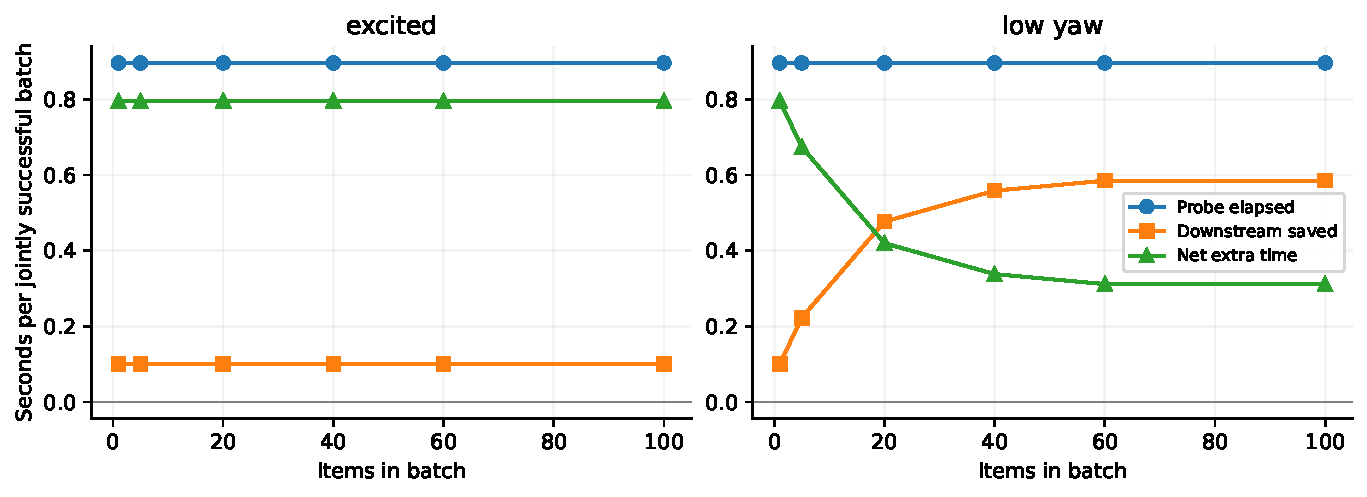
\includegraphics[width=.93\textwidth]{../revision/decomposition.pdf}
\caption{Conditional time accounting in the nominal experiment. Low-yaw downstream savings plateau; extrapolating the initial trend linearly would incorrectly predict a mean break-even beyond $N=20$. The full per-seed distribution is supplied in the artifact.}
\label{fig:decomp}
\end{figure*}

Mean probe excess stays positive through $N=100$ (Table~\ref{tab:effects}). Low-yaw savings plateau at 0.585 s, leaving 0.311 s [0.175, 0.429] excess at both $N=60$ and 100. There is no observed \emph{mean} nominal break-even in the tested range. Nevertheless, four of the 27 low-yaw scenarios benefit individually at $N=40,60,100$. Batch-aware still declines every nominal probe, missing all four: at $N=100$ it agrees with hindsight in 23/27 cases and has mean regret 0.066 s [0.013, 0.132], maximum 0.602 s. Hence equality with passive is not a certificate of optimal decisions.

At nominal $N=20$, ignore-passive and the uncertainty trigger select the probe in all 27 reached decisions and therefore exactly reproduce always-probe robot times. These are the same two physical actions, not independently different execution algorithms. The frozen-model original comparator remains slower (successful means 39.653 s exciting and 39.564 s low yaw); its original results are retained separately. This contrast does not establish superiority over a published adaptive-control method.

\subsection{A beneficial regime and its break-even neighborhood}
With tenfold sensor noise, low-yaw tasks and $N=60$, probing saves 1.052 s [0.923, 1.194] across nine jointly completing scenarios; one of ten scenarios fails before the decision. Actual probe time remains 0.896 s while downstream savings grow to 1.948 s. Batch-aware selects all nine beneficial probes, giving 9/9 decision agreement and zero two-action hindsight regret in this cell. It is now distinguishable from never-probe, whose regret is 1.052 s.

In the sequential refinement, mean net excess is 0.596 s at $N=5$, 0.349 at 10, 0.149 [0.110, 0.190] at 15, $-0.026$ [$-0.099$, 0.045] at 20, $-0.179$ [$-0.274$, $-0.087$] at 25, and $-0.319$ s at 30. Thus the sampled mean changes sign between 15 and 20; local linear interpolation suggests $N\approx19.2$, only a descriptive estimate. The $N=20$ interval includes zero; the tested cells at 15 and 25 more clearly bracket opposite signs. This is a scenario- and heuristic-dependent crossing, not a universal threshold.

The rule declines probes at $N=5,10,15$ and selects them at $N=20,25,30,60$. Near the crossing ($N=20$), only 5/9 probes are hindsight-beneficial, yet all nine are selected. Sensitivity is 5/5, specificity 0/4 and mean regret 0.040 s [0.012, 0.070]. The favorable $N=60$ result therefore does not validate calibration near the decision boundary.

\begin{figure*}[t]
\centering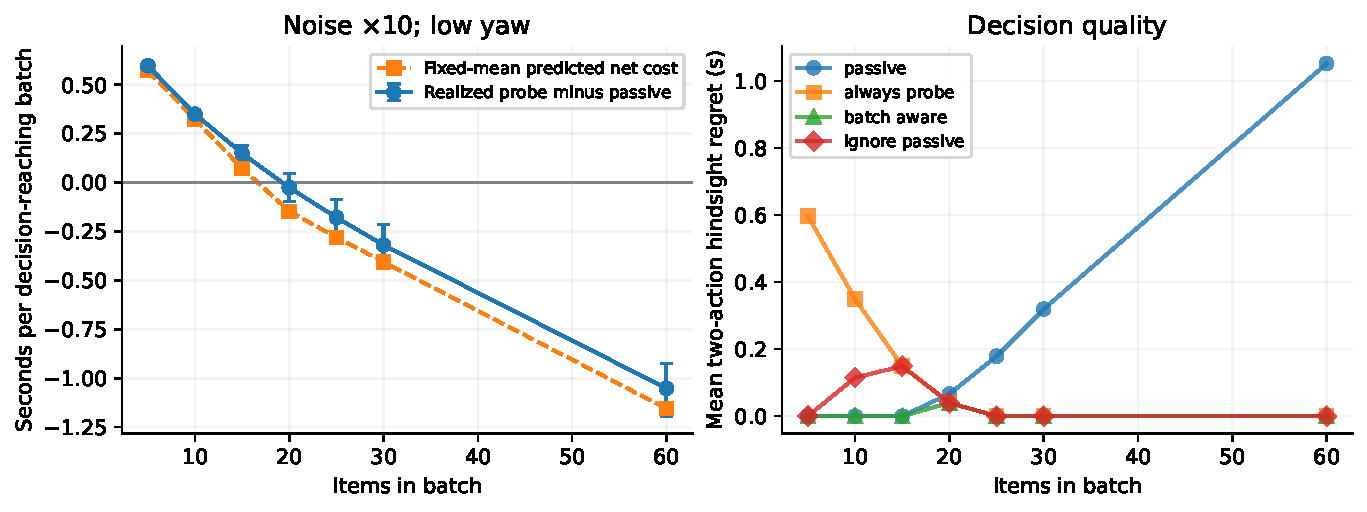
\includegraphics[width=.93\textwidth]{../revision/break_even.pdf}
\caption{Low-yaw tasks with tenfold noise. Left: measured and fixed-mean predicted net probe cost; error bars resample nine decision-reaching, jointly successful seeds. Right: two-action hindsight regret. Horizons 5, 10, 15, 25 and 30 are explicitly sequential exploratory refinements. Overlapping zero-regret traces use distinct markers; all numeric values are released.}
\label{fig:break}
\end{figure*}

\begin{table*}[t]
\centering\small
\caption{Selected low-yaw decision diagnostics. ``Beneficial'' counts paired scenarios where probe cost is lower by more than 2 ms; ``Selected'' counts probes. Regret includes a 10 s unfinished-item penalty if needed. Full results for all five decision rules, with intervals and failure counts, are in the artifact.}
\label{tab:decisions}\begin{tabular}{llrrrr}\toprule
Setting & Method & Correct & Beneficial & Selected & Regret (s)\\\midrule
base, 100 & Passive & 23/27 & 4 & 0 & 0.066\\
base, 100 & Always probe & 4/27 & 4 & 27 & 0.377\\
base, 100 & Batch aware & 23/27 & 4 & 0 & 0.066\\
noise10, 20 & Passive & 4/9 & 5 & 0 & 0.066\\
noise10, 20 & Always probe & 5/9 & 5 & 9 & 0.040\\
noise10, 20 & Batch aware & 5/9 & 5 & 9 & 0.040\\
noise10, 60 & Passive & 0/9 & 9 & 0 & 1.052\\
noise10, 60 & Always probe & 9/9 & 9 & 9 & 0.000\\
noise10, 60 & Batch aware & 9/9 & 9 & 9 & 0.000\\
margin2, 60 & Passive & 2/9 & 7 & 0 & 0.559\\
margin2, 60 & Always probe & 7/9 & 7 & 9 & 0.023\\
margin2, 60 & Batch aware & 2/9 & 7 & 0 & 0.559\\
margin4, 60 & Passive & 0/9 & 9 & 0 & 2.587\\
margin4, 60 & Always probe & 9/9 & 9 & 9 & 0.000\\
margin4, 60 & Batch aware & 9/9 & 9 & 9 & 0.000\\
\bottomrule\end{tabular}
\end{table*}

\subsection{Sensitivity and probe-induced failures}
The sign depends on the duration heuristic (Table~\ref{tab:decisions}). For low-yaw $N=60$ and the same ten seeds, halving the margin gives probe excess 0.832 s; doubling it gives $-0.536$ s [$-0.848$, $-0.217$]; quadrupling gives $-2.587$ s [$-3.015$, $-2.324$]. Batch-aware misses all seven beneficial scenarios under the doubled margin, with mean regret 0.559 s, but selects all nine under the quadrupled margin. This is a material counterexample to generally reliable value-of-information decisions. Inflation factors 4 and 64 yield excesses 0.694 and $-0.470$ s, respectively; the latter is selected correctly in all nine reached scenarios. Altering only the nominal allowance to 0.7 or 1.1 s does not change its decisions in the tested sensitivity cells.

A faster 0.3 s probe leg reduces probe time to 0.696 s but completes only 4/10 batches, compared with passive's 9/10, in each family at $N=60$. Five extra failures occur after the decision; the maximum probe acceleration ratio is 1.289. Its low-yaw conditional mean excess of $-0.099$ s is therefore not evidence of a better policy. A slower 0.6 s leg costs 1.296 s and adds 0.747 s in the low-yaw $N=60$ cell. Probe duration and allowance are changed as a declared pair, so this test does not isolate their separate causal effects. At noise scale 100, no method completes an $N=60$ batch in either family (0/10); failure-adjusted costs are retained and no conditional speed benefit is defined.

The largest logged nominal post-grasp duration margin is 0.1044 s; the initial prior value remains 0.1812 s. The screening cap never binds in the 74,580 nominal loaded-transfer schedule calls. At nominal $N=20$, passive's mean rounding residual is 15.18 ms (exciting) and 14.00 ms (low yaw). Small forecast improvements can therefore disappear under 25 ms quantization. The full sensitivity results and failure counts are supplied rather than selecting only favorable cells.

\subsection{Uncertainty forecasts and friction mismatch}
For nominal passive $N=100$, the median one-transfer predicted/realized uncertainty-scale ratio is approximately 1.000 for both parameters and families. In low-yaw tasks, the fixed-mean horizon rollout ratios are 1.048 for mass and 0.988 for inertia; mean absolute log ratios are 0.048 and 0.042. These summarize 2,700 correlated item observations from 27 scenarios, not 2,700 independent samples. Figure~\ref{fig:forecast} overlays median predicted and realized scales; per-seed traces, one-step predictions and probe-leg predictions are released. Good marginal scale prediction is insufficient to guarantee correct quantized cost decisions.

\begin{figure*}[t]
\centering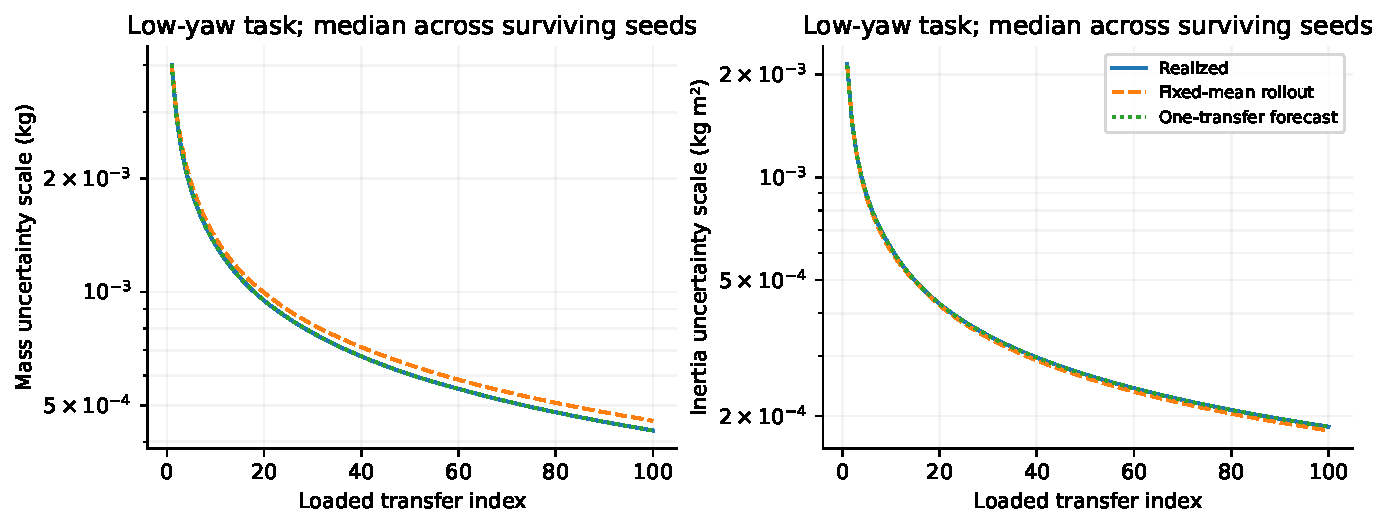
\includegraphics[width=.93\textwidth]{../revision/forecast_check.pdf}
\caption{Predicted and realized uncertainty scales for nominal low-yaw passive $N=100$. Curves are medians across 27 completed scenarios; the one-transfer predictor restarts from the current realized estimate, while the horizon rollout fixes the first post-grasp mean and omits future grasp information. These are inflated scales, not calibrated posterior standard deviations.}
\label{fig:forecast}
\end{figure*}

With matched seeds, friction multipliers 0.75, 1.25 and the asymmetric mismatch retain 27/30 completions per non-oracle method at $N=20$. Batch-aware remains identical to passive in robot time. Always-probe adds 0.796 s for exciting paths and 0.418, 0.423 and 0.421 s, respectively, for low-yaw paths. Mass-interval coverage is 3/30 per adaptive method/family (the three failed-grasp cases), and 0/27 among completed batches; inertia coverage is 30/30. The exact descriptive interval for 3/30 is [0.021, 0.265]. Nominal adaptive coverage is 30/30 per method/family/horizon for both parameters, interval [0.884, 1.000], reflecting conservative inflation rather than calibration. The original different-seed stress runs' 0/10 mass coverage has interval [0, 0.308]; their timing and cost are now included in the supplement.

The conditional-inertia physical-payload check also retains 27/30 completions; probe excess is 0.796 s (exciting) and 0.306 s (low yaw) at $N=20$. This addresses implausible independent mass/inertia combinations locally, without claiming a measured payload population.

\subsection{Numerical and artifact verification}
Two hundred random configurations pass independent energy, Christoffel, regressor and inverse/forward checks. Maximum energy discrepancy is $2.2\cdot10^{-16}$ J; Christoffel torque error is $4.0\cdot10^{-11}$ N m, with zero vertical-force discrepancy. Against independent DOP853 integration under fixed effort, maximum positional errors are $1.7\cdot10^{-15}$ rad and $1.4\cdot10^{-13}$ m; velocity errors are $1.3\cdot10^{-15}$ rad/s and $1.8\cdot10^{-12}$ m/s. Componentwise values are supplied.

Six noiseless closed-loop checks halve the plant integration step while retaining the 2 ms control period. Maximum endpoint Cartesian difference is $7.8\cdot10^{-9}$ mm, yaw difference $5.5\cdot10^{-10}$ degrees and settling-time difference zero at the scoring resolution. These are endpoint checks, not a bound on every intermediate state or on identification bias. All 6,050 revised run keys match their declared designs; frozen hashes, component-time sums and selected-action equivalence pass. Numerical consistency does not establish physical-model validity.

\section{Discussion and limitations}
The evidence now covers both costly and beneficial probing, while also exposing decision errors. The measured identity is $\Delta t_N=t_{\rm probe}-\sum_i s_i$, where $s_i$ is the paired saving in all non-probe segments of item $i$. A constant-saving approximation gives $N^*\approx t_{\rm probe}/\bar s$, but passive learning makes $s_i$ horizon-dependent and can exhaust the available savings. The nominal plateau demonstrates why this approximation cannot generally locate break-even. In the noisier setting, slower passive information accumulation leaves enough savings to repay the same probe.

The proposed rollout does not reliably track this trade-off across all conditions: it misses some nominal and doubled-margin opportunities and over-probes near a noisier crossing. An uncertainty threshold and an illustrative ablation do not constitute state-of-the-art algorithm comparisons. The contribution is the reproducible accounting framework, explicit conditioning and counterexamples, with modest methodological novelty.

Results depend on one fixed probe, two path families, exact nominal friction, idealized independent velocity sensing, the asymmetric margin and duration quantization. Sensitivity is one factor at a time, not a full interaction design. Ten-seed sensitivity cells provide limited precision, and the sequential crossing refinement is exploratory. We do not tune a replacement rule on these results or relabel reused scenarios as fresh validation. A future rule would require genuinely new scenarios and a declared evaluation protocol.

The model omits off-axis loads, compliance, backlash, motor delays, collision avoidance and contact mechanics. Instantaneous load acquisition causes startup failures; no startup safety filter is demonstrated. Sampled checks and inflated uncertainty do not give continuous-time or hardware safety guarantees. No hardware experiment or published-method reimplementation is reported.

\section{Conclusion}
A passive-learning baseline changes the economics of payload probing. Nominal mean probe overhead remains positive through 100 items, but larger noise or stronger uncertainty-to-duration coupling produces beneficial regimes. The fixed-mean rule selects some of them and fails in others. Explicit overhead decomposition, conditional timing, failure accounting and two-action regret make both outcomes visible. The results support a bounded simulation benchmark, not universal rejection of probing or general validation of the rollout policy.

\section*{Reproducibility}
The accompanying anonymous computational artifact contains source, pinned dependencies, original and post-review frozen designs, raw runs, per-item forecasts, numerical checks and manuscript sources. The command \texttt{python revision.py analyze} regenerates the revised tables and figures; \texttt{python revision.py rerun} repeats all post-review simulations after backing up existing raw files. Local hash records document execution provenance, not external preregistration. The artifact is supplied with the manuscript; no external repository URL or hardware dataset is asserted.

{\small
\setlength{\parskip}{0pt}
\bibliographystyle{unsrt}
\bibliography{references}
}
\end{document}
